\subsection{Description of the Networks}
\label{subsec:descriptionofnetwork}
As mentioned in section \ref{sec:introAndMotivation} we want to simulate the spread of opinions on a small world network. To have a comparison we also simulated the change of opinions on a random graph. Small world networks and random graphs also have a close connection as figure \ref{influencerewiringprob} shows. In this figure we visualized the Watts and Strogatz model for different rewiring probabilities. If the rewiring probability variies from 0 to 1 a regular graph passes over into a small world network and then into an random graph. In the following we are going to describe the properties of the two network types used in our model.

\begin{figure}
\centering
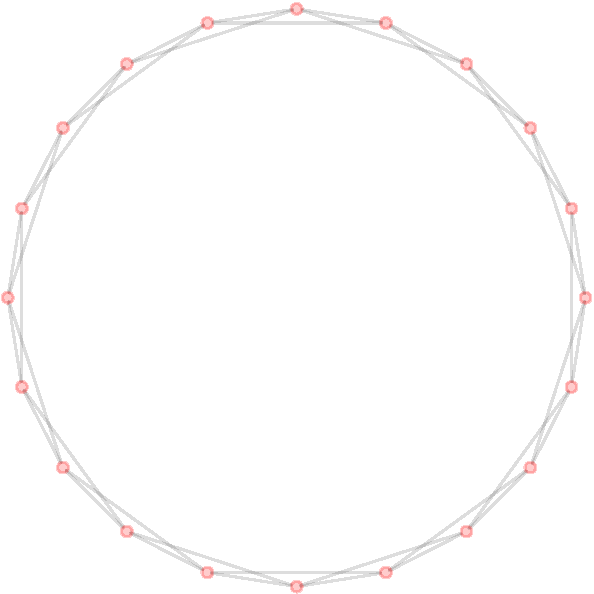
\includegraphics[width= .2 \textwidth]{Influencealphaonnetwork/networkbeta00-crop}
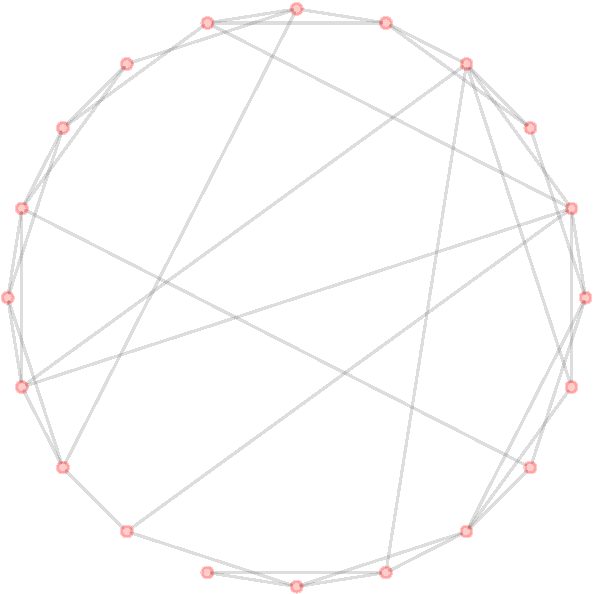
\includegraphics[width= .2 \textwidth]{Influencealphaonnetwork/networkbeta03-crop}
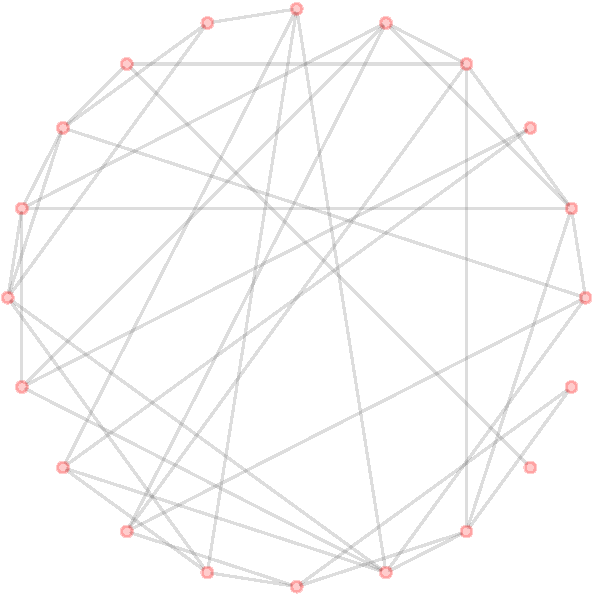
\includegraphics[width= .2 \textwidth]{Influencealphaonnetwork/networkbeta06-crop}
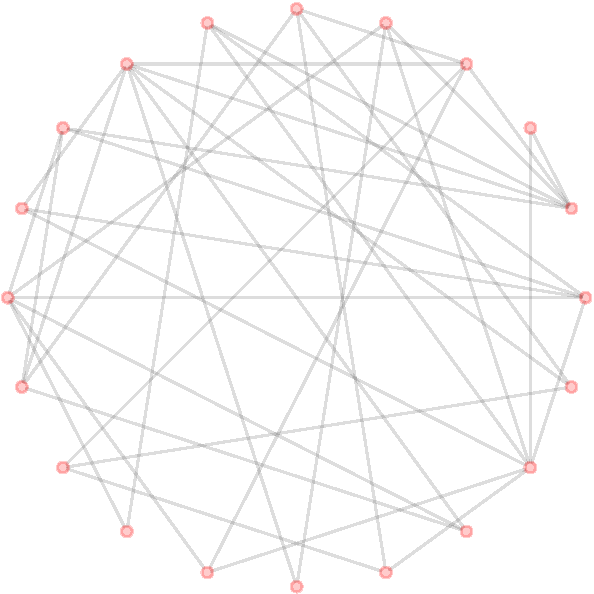
\includegraphics[width= .2 \textwidth]{Influencealphaonnetwork/networkbeta10-crop}
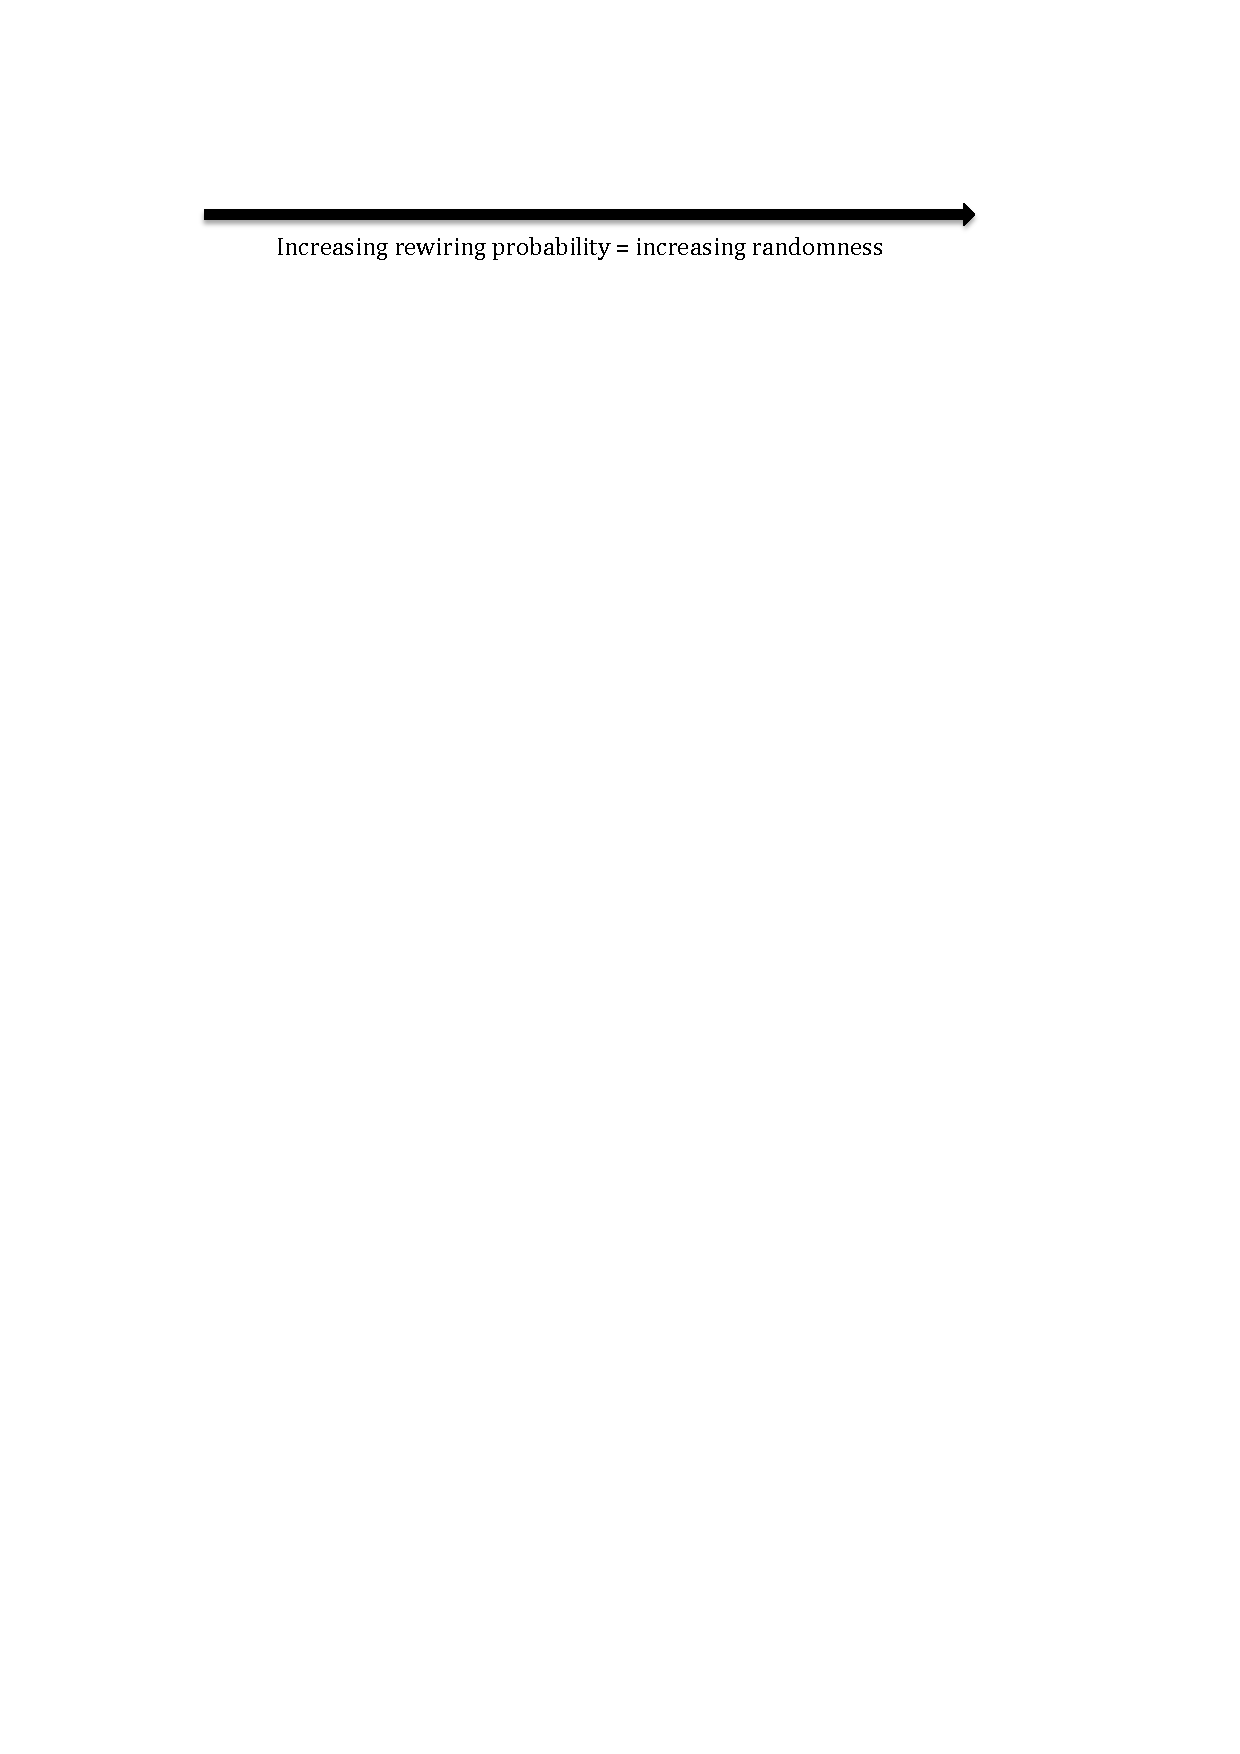
\includegraphics[width= .8 \textwidth]{Influencealphaonnetwork/arrow}
\caption{The influence of the rewiring probability varriing between 0 and 1 on a network with 20 nodes and k = 4 (graphs are generated with the use of the smallworld.m function in the appendix)}
\label{influencerewiringprob}
\end{figure}


\subsubsection{Small World Network}
\label{subsubsec:smallworld}
The most important property of an small world network is that most nodes could be reached from every other by quite a small number of steps. As described in the paper ADDREFERENCE the typical distance L of two random picked nodes is proportional to the log of the total number of nodes.
\begin{equation}
L \propto \log N
\end{equation}
In our model we use the model proposed by Watts and Strogatz. This implements the two main properties of small world networks, which are
\begin{enumerate}
\item small average path length
\item high clustering coefficient
\end{enumerate}
The Watts Strogatz algorithm follows a simple rule. As in figure \ref{influencerewiringprob} the plot on the left shows first there is a regular ring lattice constructed, where every node has exactly for a chosen integer k k neighbours. In a second step every node is taken an rewired with a chosen probability. It is done in a way avoiding loops and duplication \ie connecting a node to itself.\\
A lot of real world examples follow small world type networks. The most famous experiment showing this was done by S. Milgram showing that the average distance between two random persons in the world is five. Other examples that follow the two most important proberties of small world networks are the world wide web, social networks and for example also gene networks. \\
One of the main criticism about small world networks is that they produce unrealistic degree distributions. Many real networks follow the preferential attachement models for example proposed by Barabasi, which give us scale free networks. This means that the produced networks have hubs with a lot of links but also many nodes with just a few links to other nodes. But scale free networks fail to have a high clustering coefficient which also a lot of real world networks have. So neither of the models is perfect.

\subsubsection{Random Graph}
\label{subsubsec:randomgraph}
As the name already says random graphs are generated with some random processes. One of the most important differences of a random graph compared to a small world network is the lack of local clustering. Also the degree distribution is binomial. We used an implementation after a model proposed by $Erd\acute{o}s$ and $R\acute{e}yi$. It could be understood as the limiting case of the Watts Strogatz Algortihm described in section \ref{subsubsec:smallworld} for a rewiring probability of 1. An example is the graph on the right in figure \ref{influencerewiringprob}.